\chapter{Characterization of Coronal Bright Fronts}
\label{chapter2}

\section{Introduction}

\section{Observations}

\section{Data Analysis and Methods}

\subsection{The SPREAdFAST Framework}
The Solar Particle Radiation Environment Analysis and Forecasting-Acceleration and Scattering Transport (SPREAdFAST) framework is a physics-based global modeling framework integrates detailed Extreme Ultraviolet (EUV) observations of Coronal Mass Ejection-driven Shock and Sheath (CBF) events with modeling of the interacting coronal plasma and the subsequent production and interplanetary transport of Solar Energetic Particles (SEPs). The following sections provide a concise overview of the key components utilized in the SPREAdFAST framework for this study.

\subsection{CBF Kinematics and Geometric Modeling}
To characterize the kinematics of CBFs, we implement the methodology of the Coronal Analysis of Shocks and Waves (CASHeW) framework, as proposed by \citet{kozarev_2017}, within the SPREAdFAST framework. This methodology has been further refined and updated. Our approach aligns with the techniques presented by \citet{long_2021} and \citet{downs_2021}, where we track the leading edge of the CBF front across consecutive Atmospheric Imaging Assembly (AIA) images. Additionally, we compute the kinematics of the peak and back edge of the CBFs over time, enabling the estimation of their time-dependent mean intensity and thickness.

Figure~\ref{fig1} exemplifies the application of this methodology to the CBF event on May 11, 2011. Panel A displays a mid-event AIA 193-channel base difference image, clearly illustrating the CBF. Radial and lateral lines of measurement are overlaid on the image. The kinematics are determined through time-height maps, commonly known as J-maps \citep{sheeley_1999}. These maps are generated by stacking columns of pixels in a desired direction from a solar image. The track's shape on J-maps depends on the feature's direction and speed, allowing identification of radial and lateral wave front positions over time. The radial direction measurements (Panel B) are taken along the line passing through the solar center and the CBF nose (predominant direction of motion). Lateral wave front signatures are measured in two directions away from the radial direction (Panels C and D), parallel to the solar limb. The lateral measurements in both directions are averaged to form a single lateral kinematics time series for each event. The resulting CBF width and mean intensity in both directions are also recorded.

To obtain the kinematics in the AIA field of view (FOV), a Savitzky-Golay fit is applied, following the method proposed by \citet{kozarev_2019}. The smoothed positions are then extrapolated to 10\rsun using the analytical model of \citet{byrne_2013}. Based on the measured front positions over time, a three-dimensional, time-dependent geometric spheroid model named Synthetic Shock Model (S2M) is developed for all compressive fronts. This model, consisting of over 1000 points, is utilized to estimate the dynamic shock upstream coronal parameters. Figure~\ref{fig2} illustrates 9 time steps of the S2M for an eruption near the northwest limb of the Sun.
The spheroid, centered on the eruption source, maintains its aspect ratio throughout the event. Once the S2M wraps around the Sun, points behind the plane passing through the eruption source point, and perpendicular to the radial direction at that point, are removed from consideration. The S2M is divided into a cap and two side zones, denoted by blue, green, and red points in Figure~\ref{fig2}. This division allows for the investigation of variations in the plasma environment as the CBF traverses in the radial and lateral directions.
The \textit{nose} of the shock model is defined as the collection of all model points on the spheroidal cap subtending a half-angle of $\pi$/7 from the semi-major axis of the spheroid at each time step. The remaining points on the shock surface are divided into two flanks or zones, with the dividing plane parallel to the Sun-Earth line. Plasma parameters at points on these three surfaces can be examined separately, providing insights into the differences in the plasma environment through which the CBF passes, as demonstrated in Figure~\ref{fig2}.






\section{Results and Discussion}

\section{Conclusions}




%%%%%%%%%%%%%%%%%%%%%%%%%%%%%%%%%%%%%%%%%%%%%%%%%%%%%%%%%%%%%%%%%%%%%%%%%%%%%%%%%%%%%%%%

\section{Wavetrack: A Flexible Framework for Automated Recognition and Tracking of Wave-Like Events in Solar Imagery}
\subsection{Overview}
Solar eruptive events encompass a myriad of intricate phenomena, including flares, filament eruptions, coronal mass ejections (CMEs), and CME-driven shock waves. The principal drivers of solar energetic particles (SEPs) are acknowledged to be CME-driven shocks within the corona and interplanetary space. This acceleration primarily occurs through the diffusive shock acceleration (DSA) and shock drift acceleration (SDA) processes \citep{reames_2021}. Efforts have been devoted to characterizing and modeling SEP acceleration under ideal conditions \citep{vainio_2008, sokolov_2009, kozarev_2013}. Recent endeavors have shifted towards the development of more realistic CME-shock and SEP acceleration models, incorporating observational data \citep{vourlidas_2012, kwon_2014, kozarev_2015, kozarev_2019}.

Understanding the efficiency and spatial distribution of SEP acceleration necessitates a comprehensive grasp of CME-shock interactions with three-dimensional coronal fields \cite{rouillard_2016}. The modeling of DSA requires the deduction of shock front shapes from observations, given the profound impact of the local magnetic field-shock angle on acceleration \cite{guo_2013}. Moreover, the lateral over-expansion of CMEs early in their evolution modifies the compressive front \cite{bein_2011, temmer_2016}, necessitating improvements to the idealized shock surface descriptions used in modeling \citep{vourlidas_2012, kwon_2014, rouillard_2016}.

The utilization of extreme ultraviolet (EUV) imaging, facilitated by instruments such as STEREO/EUVI \citep{wuelser_2004} and SDO/AIA \citep{lemen_2012}, enables the characterization of shocks. The high resolution and multi-wavelength coverage of these instruments permit the time-dependent modeling of SEP acceleration \citep{kozarev_2016, kozarev_2017, kozarev_2019}. With the burgeoning demand for Big Data, solar feature detection has become more automated, employing fundamental techniques reviewed by \citet{aschwanden_2010} and applied to features at various heights \citep{perez_Suarez_2011}. Some of these techniques are tailored to detect specific solar features, such as sunspots and active regions \citep{curto_2008}.

EUV wave recognition and tracking pose challenges due to their weak intensity in proximity to other features. While algorithms for this purpose exist, their complexity is notable \citep{podladchikova_2005, verbeeck_2014, long_2014, ireland_2019}. Specifically, CorPITA \citep{long_2014} and AWARE \citep{ireland_2019} fit shapes to flare-centered wave sectors but are constrained to the solar disk.

This study, led by \citet{stepanyuk_2022}, introduces Wavetrack, a flexible, object-oriented Python library designed for general solar feature detection and tracking. Wavetrack integrates multiscale representation \citep{starck_2002}, \'A trous wavelets \citep{akansu_1991, holschneider_1989}, and filtering at its core. Notably, Wavetrack has the capability to generate training sets for machine learning-based recognition.

Machine learning applications are gaining prominence in solar physics, spanning areas such as EUV irradiance mapping \citep{szenicer_2019}, solar flare prediction \citep{li_2013}, and magnetic flux generation \citep{kim_2019}. However, the potential of data-driven CME tracking is hindered by limited training sets. Wavetrack addresses this limitation by facilitating the conversion of results into annotated sets.

Central to Wavetrack is a method for general feature recognition and tracking, implemented as an accessible, open-source Python library. Its modular structure allows the configuration of applications by adjusting a few threshold parameters. The calculation scheme integrates multiscale data representation \citep{starck_2002} and the \'A trous wavelet transform \citep{akansu_1991, holschneider_1989}, supplemented by image filtering techniques for noise removal and edge enhancement.

Wavetrack distinguishes itself from existing algorithms by offering a flexible framework for detecting various solar features in EUV, white light, and other observations. Its modular design facilitates the generation of training sets for machine learning approaches, supporting automated analysis for deriving new insights from the extensive solar data. The \'A trous wavelet transform' employed by Wavetrack enables the isolation of features at different scales, effectively separating noise from the signal and enhancing edges. Wavelet coefficients encode the multiscale structure efficiently, with thresholding suppressing noise by zeroing insignificant values. Further refinement of the signal is achieved through filtering techniques. Morphological operations, such as opening, eliminate artifacts and smooth edges, while contrast enhancement sharpens edges and boundaries. The resulting output highlights features while suppressing noise.

Wavetrack strategically applies these techniques to recognize faint features like EUV waves and tracks them by identifying significant coefficients across wavelet scales. This approach avoids pre-processing steps, such as difference images, that may introduce false signals. The adaptability of Wavetrack is a key feature, allowing users to build specific applications by adjusting parameters such as thresholds and filters. Importantly, the original data remains unaltered, with only processed copies utilized for feature detection to prevent information loss.

Wavetrack, offered as an open-source tool, invites community involvement, enabling users to contribute modules, optimizations, and new techniques. This collaborative effort is poised to enhance solar data analysis capabilities in the era of Big Data, facilitating the discovery of new knowledge to deepen our understanding of the dynamic Sun.

%\subsection{Methods}
In the realm of solar image processing and analysis, diverse techniques contribute significantly to understanding solar phenomena. This section delineates the methods employed, encompassing wavelet transform, image filtering, feature detection algorithms, machine learning, and solar feature tracking.

\begin{itemize}
	\item \textbf{Wavelet Transform}:
	The application of the \'A trous wavelet transform' constitutes a fundamental multi-scale data representation concept widely employed in solar image analysis. This method facilitates the extraction of features at various decomposition and intensity levels, contributing to the comprehensive understanding of solar events.
	
	\item \textbf{Image Filtering}:
	Various image filtering techniques play a crucial role in enhancing and extracting specific features within solar images. These techniques, adept at detecting and tracking phenomena like CME shock waves and filaments, contribute significantly to the analysis of solar dynamics.
	
	\item \textbf{Feature Detection Algorithms}:
	Automated algorithms, leveraging image processing techniques, are instrumental in detecting and identifying diverse solar features, including sunspot groups, active regions, and eruptive fronts. These algorithms enhance the efficiency of solar feature identification across different types of observations.
	
	\item \textbf{Machine Learning}:
	The integration of machine learning methods, such as Convolutional Neural Networks (CNNs) and Generative Adversarial Networks (GANs), signifies a contemporary approach in solar image analysis. These methods find application in tasks ranging from predicting solar flares to generating magnetic flux distributions, enriching the analytical capabilities of solar researchers.
	
	\item \textbf{Solar Feature Tracking}:
	An essential facet of image analysis involves tracking the evolution of solar features over time. Tracking algorithms, instrumental in monitoring the movement and changes in features like CMEs, filaments, and EUV waves, contribute significantly to understanding dynamic solar processes.
\end{itemize}

The present study leveraged observations from the Atmospheric Imaging Assembly (AIA) instrument on the Solar Dynamics Observatory (SDO). The AIA instrument, functioning as an extreme ultraviolet (EUV) imager, offers high-resolution and high-temporal observations, particularly useful for detecting and characterizing large-scale shocks known as EUV waves or Coronal Bright Fronts (CBFs). Focusing specifically on the AIA channels centered on 193Å and 211Å wavelengths, the study utilized a standard AIA pipeline with the SunPy package to process the 193\AA data.

The processing involved the creation of base images through the averaging of a series of images preceding the eruption. Subsequent construction of base difference images, achieved by subtracting the base images from the current raw image sequence, facilitated the enhancement of intensity changes caused by CBFs while mitigating static details and reducing noise. Given the typically dim nature of CBFs in EUV images, the study pre-selected a segment of the dynamic range where the shock wave is revealed from the base difference image of the sequence. The observations obtained from the SDO/AIA telescope were instrumental in studying and tracking the CBFs and their temporal evolution, providing essential data for analyzing the spatial and temporal relationships of CBFs and other solar dynamic features.

\subsection{Image Filtering Techniques}
Specific image filtering techniques, including thresholding, wavelet decomposition, and segmentation, formed the cornerstone of the method. Initial thresholding applied to the absolute values of pixels in the base difference images narrowed the dynamic range, concentrating on the segment containing the object of interest.

Subsequent to thresholding, the base difference images underwent \'A trous wavelet decomposition into multiple scales. Each wavelet coefficient underwent relative thresholding based on the statistical distribution of pixel intensities at each decomposition level. The segmentation process yielded object masks for each time step, subsequently multiplied by the original data to reveal the intensity of different parts of the object.

Given the variations in statistical distributions of pixel intensities in base and running difference images, tailored approaches were applied. In base difference images, pixel intensities were constrained to a specific segment, focusing on the object of interest, such as a CBF. Running difference images, employed to identify eruption initiation, depended on the specific features and objects under observation.

The \'A trous wavelet transform, constituting a multi-scale data representation, significantly contributed to the recognition and tracking of solar images. This hierarchical decomposition enabled the extraction of specific objects and their masks from imaging observations, facilitating their tracking and temporal evolution. The \'A trous wavelet decomposition enhanced the clarity and intensity of faint features like EUV waves, offering a flexible framework applicable to various solar phenomena across different wavelengths. This method emerges as a valuable tool for comprehensively analyzing and understanding the dynamics of solar features, including CME shock waves and filaments.

The study introduced the Wavetrack package, designed for automated detection and tracking of dynamic coronal features in solar observations. Utilizing wavelet decomposition, feature enhancement and filtering, and object recomposition, Wavetrack identified and tracked features such as CBFs and eruptive filaments. This object-oriented Python framework, adaptable to both on-disk and off-limb features, enables tracking of features that bifurcate over time.

\subsection{Wavetrack for Coronal Wave Tracking}
In tracking coronal waves, Wavetrack utilized wavelet decomposition, feature enhancement, and filtering techniques. The \'A trous wavelet decomposition method enhanced faint features like EUV waves, capturing different scales of features through convolutions. Automated feature recognition, incorporating intensity thresholding, image posterization, median filtering, segmentation, and intensity level splitting, identified and isolated coronal wave features. The output comprised time-dependent pixel masks, representing the tracked coronal wave, applicable to generating final feature maps for both on-disk and off-limb features.

\subsection{Wavetrack for Filament Tracking}
For filament tracking, Wavetrack followed a process involving wavelet decomposition, feature recognition, object mask generation, and image recomposition. The \'A trous wavelet decomposition identified different scales of features, and subsequent processing enhanced the features for ease of tracking. Object masks generated for each time step isolated filament features, and image recomposition from weighted wavelet scales produced final feature maps. The choice of images, such as inverted AIA 193Å images, depended on source data and filament velocity.

\subsection{Fourier Local Correlation Tracking (FLCT) Model}
To determine the plane-of-sky velocity and speed of solar features, the study employed the FLCT model, utilizing the Fourier Local Correlation Tracking (FLCT) method. Through the analysis of consecutive solar images and the tracking of feature motion over time, the FLCT algorithm was applied to object masks derived from the Wavetrack methodology. The resultant output furnished detailed maps of instantaneous velocity, contributing to a deeper understanding of the expansion and evolution of solar features such as Coronal Bright Fronts (CBFs) and erupting filaments.

The overall methodology of the study integrated advanced image processing techniques, incorporating wavelet transform, image filtering, feature detection algorithms, and machine learning. This comprehensive approach facilitated an in-depth analysis of solar observations. Notably, the Wavetrack package emerged as a versatile tool, specifically valuable in the tracking of dynamic coronal features. Its application provided significant insights into the intricate dynamics governing the solar environment.

\subsection{Results}
The study presents several examples and case studies that demonstrate the application of the Wavetrack package. Here are some of the examples mentioned:

\begin{enumerate}
	\item \textbf{May 11, 2011 event}:
	The Wavetrack algorithm was used to track both an erupting filament and the coronal bright front it drives. The relationship between the driver and wave was studied using the segmented features from AIA 193\AA observations.
	
	\item \textbf{September 29, 2013 event}: Wavetrack was applied to a large-scale filament in a slow eruption. The segmented filament feature was overlaid on the solar corona, and the on-disk feature was consistently tracked during the eruption.
	
	\item \textbf{December 12, 2013 event}: Wavetrack was used to track the evolution of driven and non-driven regions of the CBF. The method revealed the relation between the CBF and eruptive features. These examples demonstrate the versatility of Wavetrack in recognizing and tracking various solar features, both on the solar disk and off the solar limb.
	
	\item \textbf{June 07, 2011 event}: For this event, the variation in speed between the geometric center and center of mass is up to 300 \kms in the radial direction. The angle between the geometric center and center of mass changes quite a lot as different parts of the compressive front brighten and dim. However, the angle remains relatively stable, changing only slightly during this event.
\end{enumerate}

Here, I will just focus on the first event since it was accompanied with a coronal bright front.

The Wavetrack methodology was applied to analyze three previously investigated eruptive events observed by the AIA telescope \citep{kozarev_2015, kozarev_2017}. In the first event on May 11, 2011, an erupting filament induced a relatively bright Coronal Bright Front (CBF) on the northwest region of the solar disk near the limb. The second event, occurring on June 07, 2011, originated close to the southwest limb and featured a large and luminous CBF. On December 12, 2013, the third event, also originating near the southwest limb, was examined.

Figure 4 illustrates the successfully extracted Wavetrack CBF objects for the three events, observed at four time points, each separated by 3 minutes. Wavetrack object masks, when applied to base difference images, were visualized using a blue-green color map overlaid on the original AIA 193\AA observations in grayscale to emphasize the CBFs. Across all three events, Wavetrack adeptly delineated the extent of the CBF in consecutive time steps, demonstrating its ability to track the evolution of CBFs both on the solar disk and off the limb. This capability was maintained despite the distinct pixel distributions and intensities in these two regions. The application of Wavetrack facilitated the detailed study of the time-dependent shapes and changing intensity distributions of CBFs, separate from the broader corona. Moreover, Wavetrack effectively selected CBF objects under different coronal activity states. For instance, despite increased coronal activity on December 12, 2013, Wavetrack successfully segmented the CBF. Importantly, the segmentation of the CBF in the last event highlighted Wavetrack's capability to track multiple separate parts of the same feature.

\begin{figure}
	\centering
	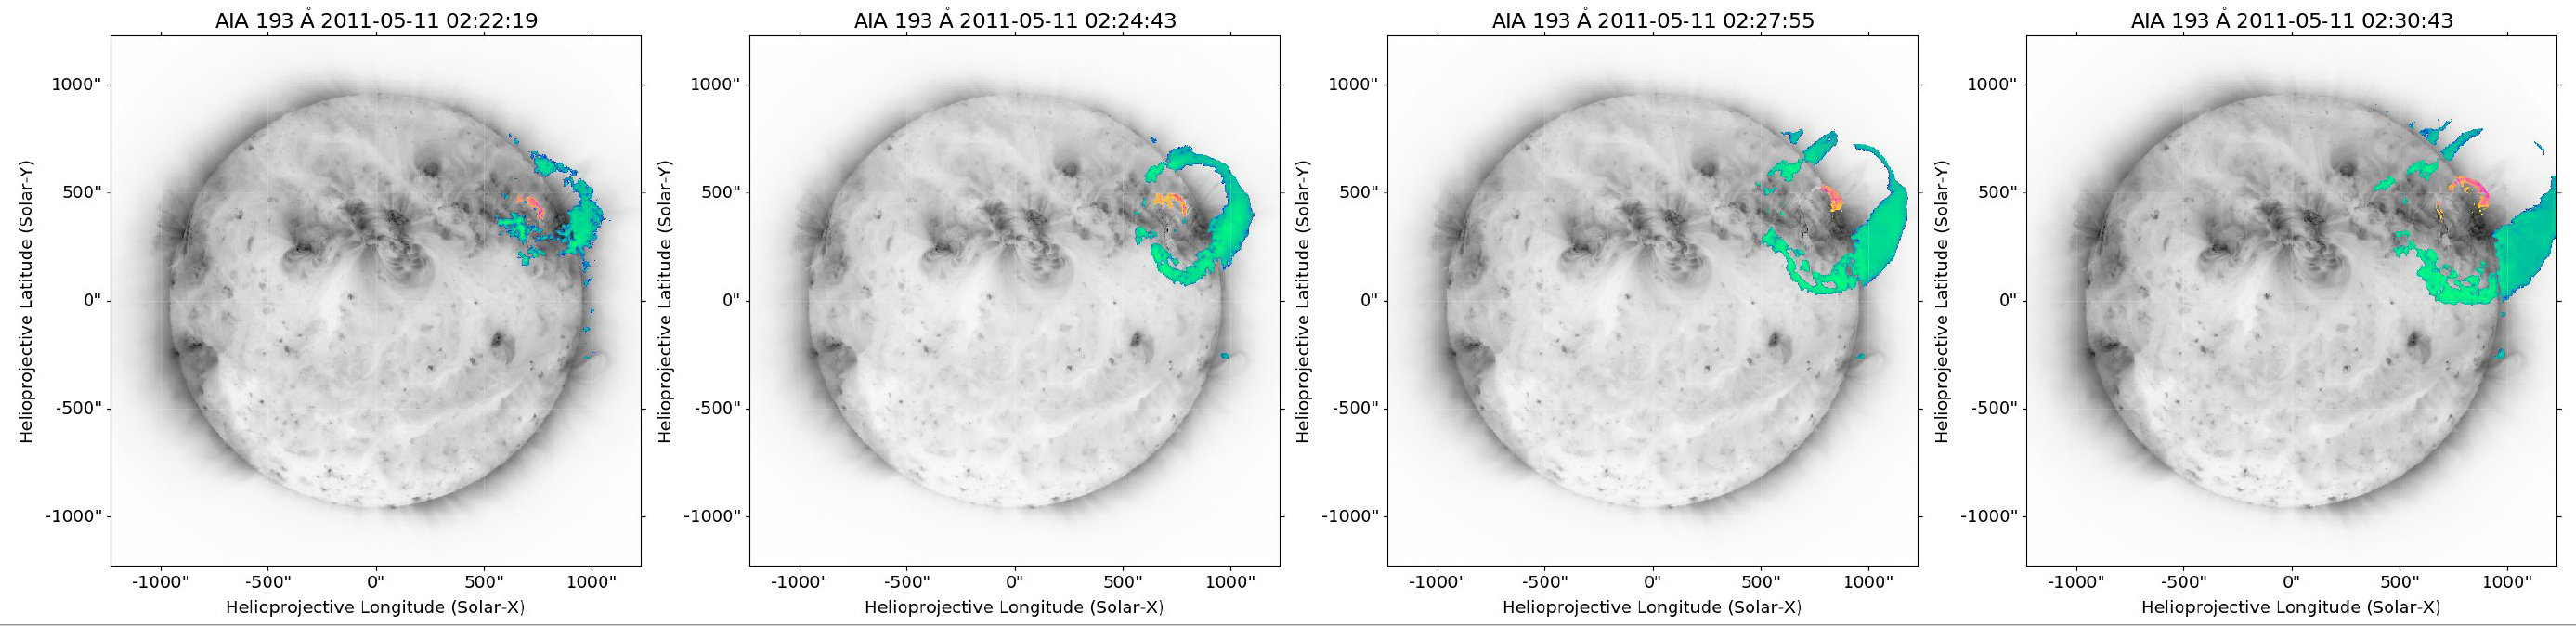
\includegraphics[width=0.9\hsize]{chapter2/figs/fig_1105011_wave_filament_fourpanel_plot.png}
	\caption{Wavetrack images showing progression of a CBF and filament on May 11, 2011. Three snapshots captured \almost2 minutes apart track the CBF and filament over time. Credit goes to \citet{stepanyuk_2022}.}
	\label{fig_wavetrack_cbf_filament}
\end{figure}

\begin{figure}
	\centering
	\includegraphics[width=0.7\hsize]{chapter2/figs/wavetrack_figure_110511.png}
	\caption{Wavetrack images of a May 11, 2011 eruption, with CBF mask applied. Four image pairs shown, separated by 2 minutes, to track CBF over time. Credit goes to \citet{stepanyuk_2022}.}
	\label{fig_wavetrack_cbf_center}
\end{figure}

The Wavetrack code was further applied to isolate and study the kinematics of CBFs and filaments in detail. The Fourier Local Correlation Tracking (FLCT) method, extensively utilized for estimating horizontal flows in photospheric magnetograms, was employed for this purpose. Initially proposed as a cross-correlation technique for precise motion measurement, FLCT calculates a 2D flow field that best resembles the scalar field between two consecutive 2D maps.

Figure 7 displays four pairs of consecutive AIA images from the May 11, 2011 event, used as input for the FLCT algorithm. Each pair, separated by 24 seconds, is strategically chosen to observe the CBF progression over 6 minutes. The corresponding FLCT results, presented in Figure 8, show the instantaneous plane-of-sky direction of motion and speed of each CBF region. Notably, the results reveal the uneven expansion of the CBF from the central source. In this event, the thinnest part of the CBF, strongly driven by the erupting filament, exhibited the fastest motion compared to other regions on the disk and off the limb. This nuanced information, not discernible from intensity observations alone, underscores the value of our combined Wavetrack and FLCT approach in elucidating the dynamic behavior of coronal features.

\begin{figure}
	\centering
	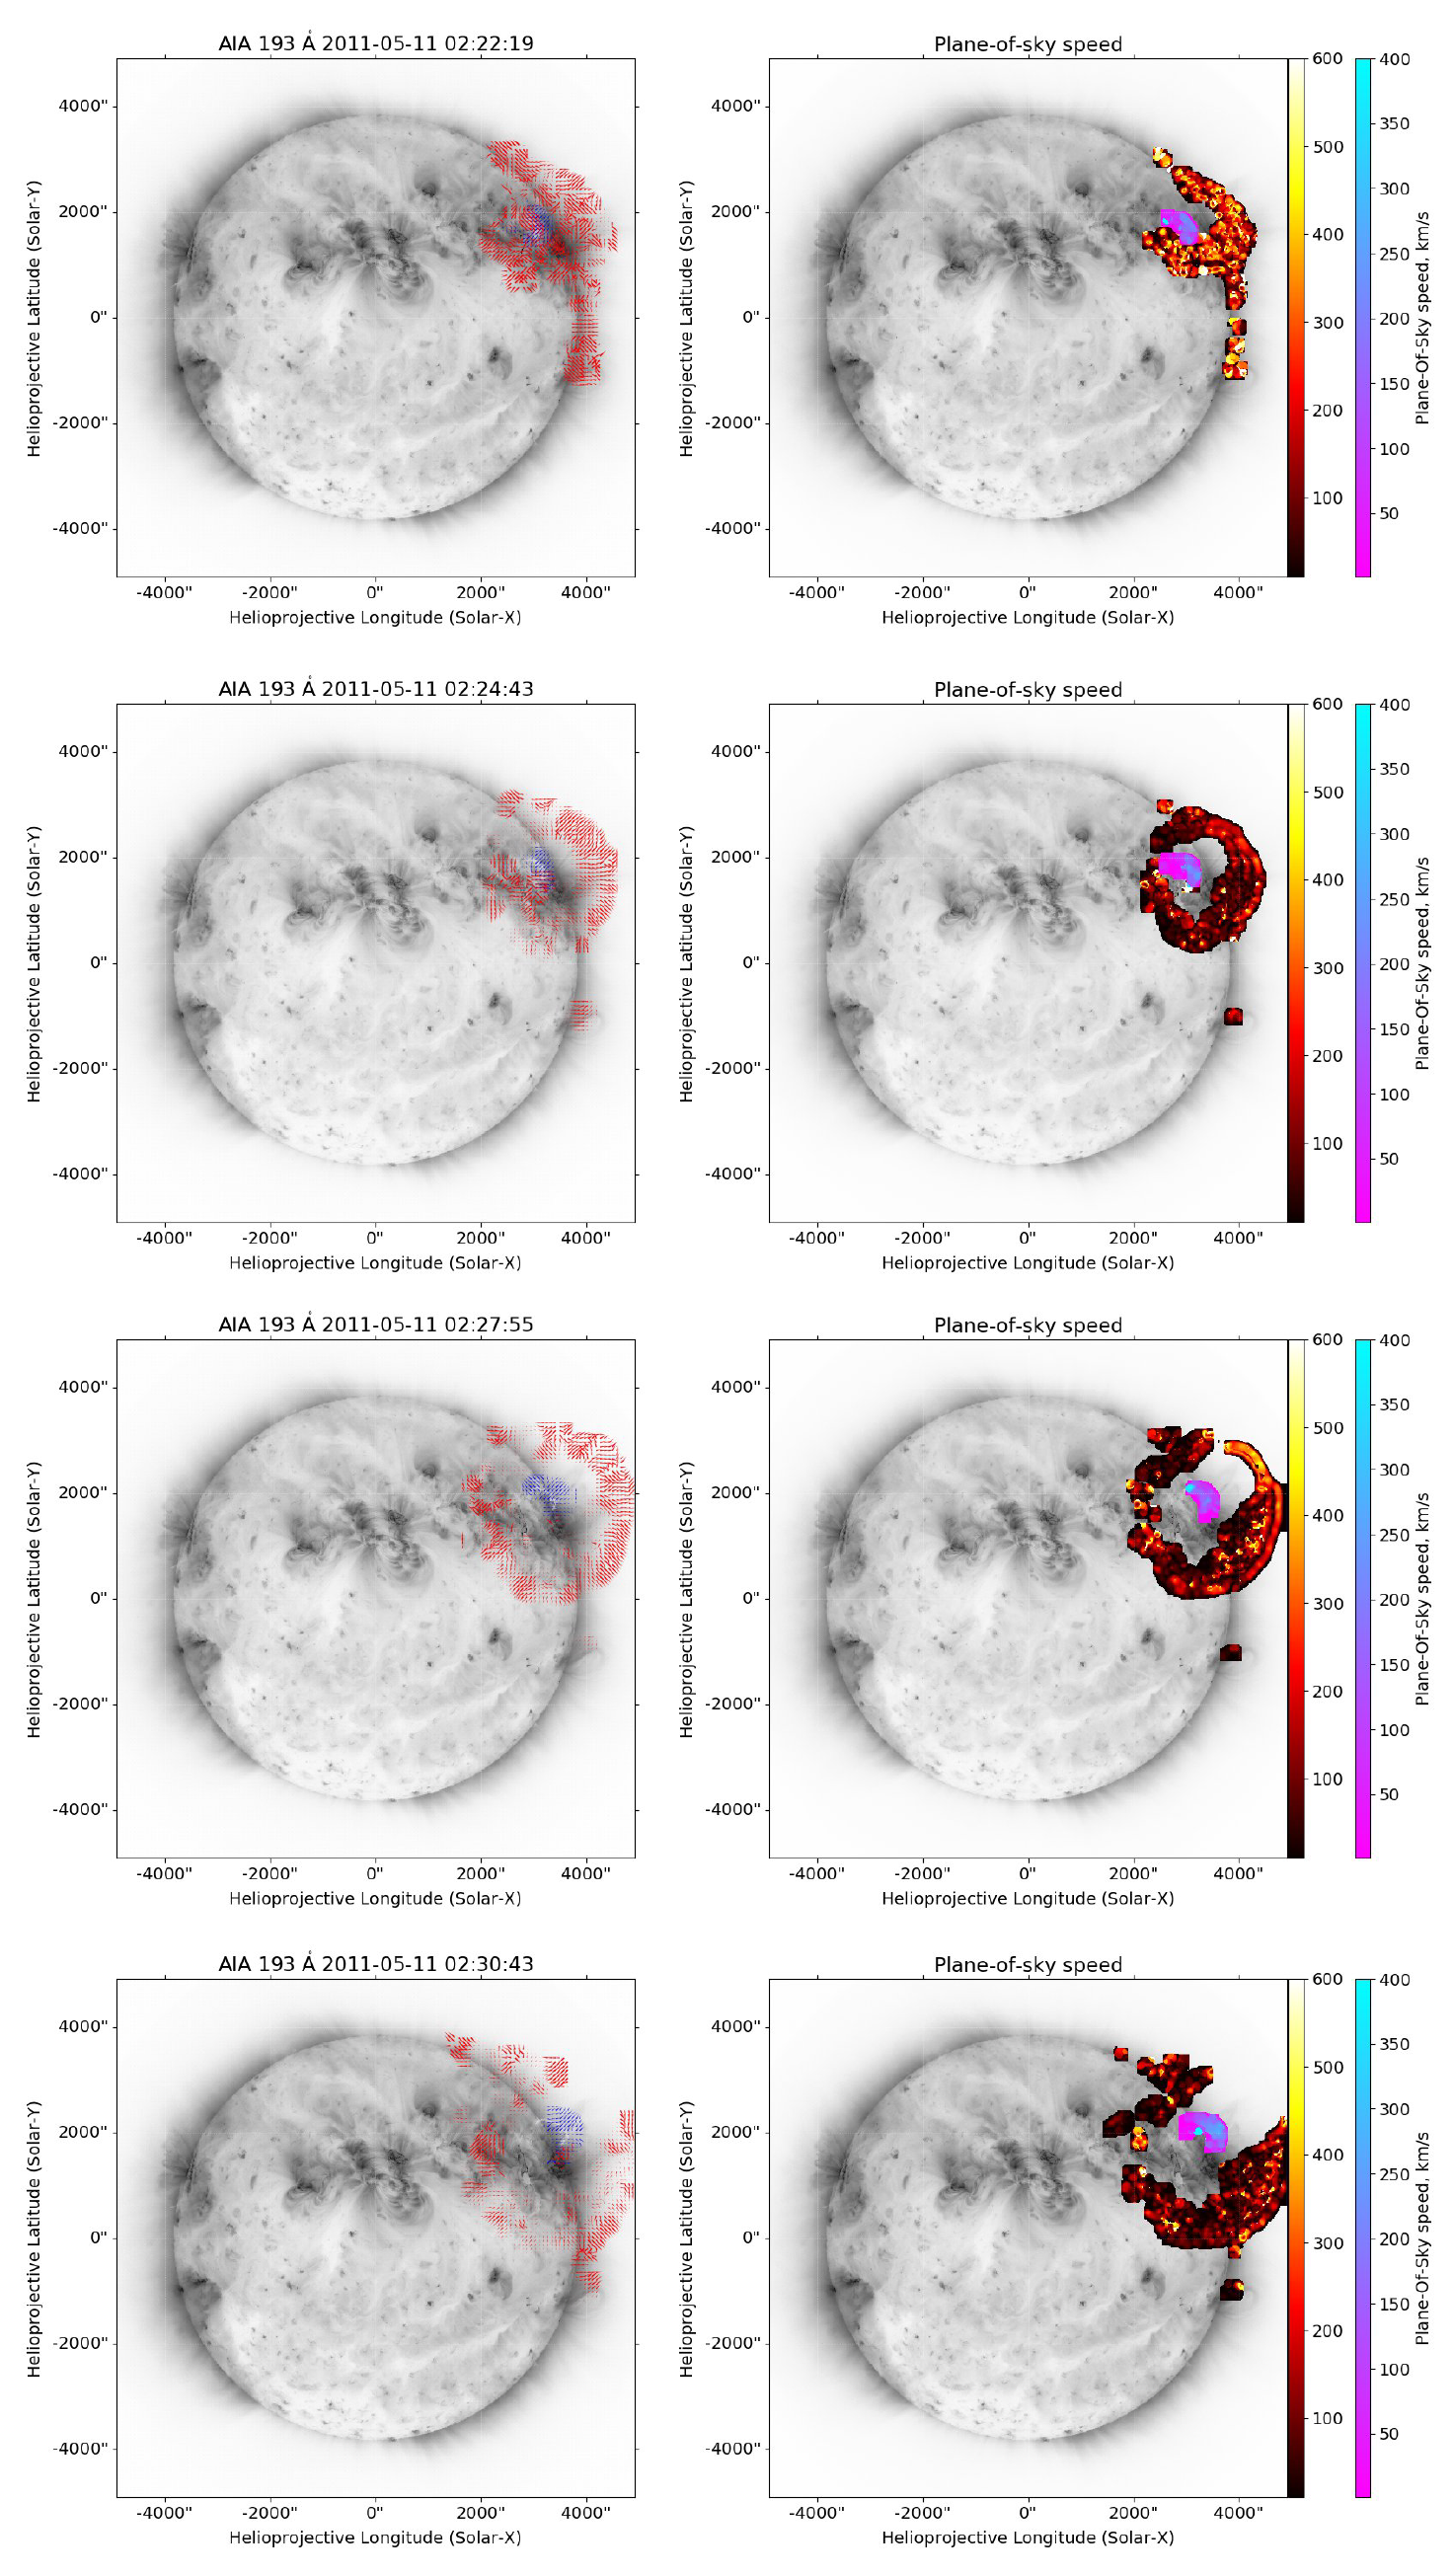
\includegraphics[width=0.7\hsize]{chapter2/figs/flct_wave_filament_doubleplot_figure_110511.png}
	\caption{FLCT model output for four image pairs from Fig. 3. Left: the plane-of-sky velocity vectors. Right: plane-of-sky speed. Credit goes to \citet{stepanyuk_2022}.}
	\label{fig_flct_110511}
\end{figure}

\subsection{Conclusions}
In this study, led by \citet{stepanyuk_2022}, we introduce Wavetrack, an innovative approach designed for the automated identification and monitoring of dynamic coronal phenomena. Employing wavelet decomposition, feature enhancement, filtering, and ultimate object recomposition, Wavetrack generates time-dependent masks for feature pixels. These masks can be applied to integral or base-difference images, yielding comprehensive feature maps. Notably, Wavetrack excels in tracing pixels associated with faint, large-scale features, such as coronal bright fronts/EUV waves in AIA observations, and has demonstrated efficacy in tracking eruptive filaments.
Operable for both on-disk and off-limb features, Wavetrack adeptly follows features that evolve into distinct components over time. Implemented as a versatile, object-oriented framework in Python, Wavetrack is freely accessible for download and utilization.

The application of Wavetrack to four distinct events, with emphasis on three – the CBFs occurring on May 11 and June 07, 2011, and December 12, 2013 – reveals its proficiency in tracking complete CBF pixel maps. These model results, when integrated with the FLCT method for calculating plane-of-sky speeds, unveil the dynamic evolution of driven and non-driven regions within CBFs, as well as their correlation with eruptive filament drivers. Our findings indicate that drivers induce a compression effect, causing CBF thinning and increased speed, aligning with theoretical models. However, the brightness of CBFs in the driven regions, as observed in AIA data, does not necessarily exhibit a significant increase.

Furthermore, Wavetrack facilitates the tracking of temporal changes in feature regions by computing the time-dependent vector between the pixel geometric center and the center of mass, determined by weighing the observed pixel intensities. This proves particularly valuable for large-scale features like CBFs, providing a straightforward metric in the form of a one-dimensional time series for characterizing feature evolution.

While the method demonstrates widespread applicability to various solar dynamic features and observational data, it currently relies on human input for the segmentation of specific feature types, particularly dim ones. Manual setting of object criteria, including threshold intervals and recomposition weight coefficients, is necessary. In instances of base difference imaging, precise selection of the base image is crucial to prevent contamination of input data with spurious features. Additionally, parameter fine-tuning through trial and error may be required for specific events. These limitations are acknowledged, and future work will address them to enhance the model's versatility.

The methodology holds promise for extensive application across diverse solar dynamic features and observational datasets. Subsequent research endeavors will extend its use to in-depth studies of filament evolution and coronagraph data. The objective is to refine our comprehension of how large-scale eruptive fronts manifest variations across distinct observational contexts, spanning the low and middle corona.
%%%%%%%%%%%%%%%%%%%%%%%%%%%%%%%%%%%%%%%%%%%%%%%%%%%%%%%%%%%%%%%%%%%%%%%%%%%%%%%%%%%%%%%%

\section{Geomagnetic Storms: CME Speed De-Projection vs. In Situ Analysis}
This study, led by \citet{miteva_2023}, examines the relationship between the intensity of geomagnetic storms (GS) and parameters of solar and interplanetary phenomena. We utilize the recently developed PyThea framework to reconstruct the 3D geometry of geo-effective CMEs and compare on-sky and de-projected values, focusing on the reliability of the de-projection capabilities. Spheroid, ellipsoid, and graduated cylindrical shell models are used. We collected parameters of the GS-associated phenomena. Considerable variation in 3D de-projections of CME speeds was obtained depending on the reconstruction model chosen and subjective observations. Fast CME speeds combined with frontal magnetic structure orientation when reaching Earth's magnetosphere proved the best indicator of GS strength. More accurate estimations of geometry, direction, and de-projected speeds are critical for operational GS forecasting in space weather prediction schemes.

\subsection{Overview}
Solar eruptive events like coronal mass ejections (CMEs) and solar flares (SFs) can generate disturbances that propagate through interplanetary space and impact Earth's magnetosphere, leading to space weather effects \citep{fletcher_2011, webb_2012, klein_2017, temmer_2021}. The electromagnetic radiation from SFs arrives at Earth first, followed by energetic particles. The plasma clouds of CMEs take longer, from tens of hours up to a few days, to impact Earth's environment \citep{malandraki_2018, gopalswamy_sun_sw_2022}. The temporary disruption of Earth's magnetosphere and atmosphere due to these solar events are known as geomagnetic storms (GSs) \citep{gonzalez_1994, saiz_2013, lakhina_2016}.

The coupling between solar wind plasma and Earth's magnetosphere occurs through magnetic reconnection, enabled when the interplanetary (IP) magnetic field turns southward (negative Bz component) and impacts Earth at high speed, as during CMEs \citep{dungey_1961, akasofu_1981, echer_2022}. This leads to increased particle injection into the magnetosphere and atmosphere, causing bright auroral displays. Drifting electrons and protons also drive the westward ring current responsible for decreases in the horizontal magnetic field measured by the disturbance storm time (Dst) index \citep{gonzalez_1994, saiz_2013, lakhina_2016}.

Fast CMEs propagating through IP space (ICMEs) cause the most intense GSs, with sudden Dst decreases, compared to gradual storms from corotating interaction regions (CIRs) \citep{tsurutani_1997, zhang_2007, wu_2016, borovsky_2006}. ICME shock waves and magnetic ejecta produce cascading effects in near-Earth space that can disrupt technology \citep{pulkkinen_2007}.

Earth-directed fast ejecta with strong southward magnetic fields inside are the most geoeffective. However, single spacecraft observations are limited by projection effects, leading to uncertain CME speed estimations \citep{paouris_2021, kouloumvakos_2022}. Previous studies found no clear relationship between GS intensity and solar flare parameters or CME properties like projected speed and angular width \citep{samwel_2023}. Furthermore, CME magnetic structure cannot be derived from remote sensing data. Reliable solar or near-Sun measurements that provide early warnings for potential GS strength remain lacking.

Accurately predicting when an incoming disturbance will impact Earth requires determining the arrival time and speed of CMEs. Different portions of these large structures, such as the apex or flanks, can hit Earth upon arrival at 1 AU. Flank hits may only involve the CME sheath while apex hits include both sheath and ejecta, leading to different magnetospheric effects \citep{kay_2018}. Therefore, deducing CME directionality and 3D geometry is important. To maximize forecast lead time, these parameters should be estimated as early as possible when the CME emerges in coronagraph fields of view. In images, CMEs appear as line-of-sight integrated brightness enhancements projected onto the observing plane \citep{vourlidas_2003, jackson_2010}.

Further developing reconstruction techniques to correct for projection effects can improve CME propagation understanding and impact forecasting \citep{thernisien_2009, mierla_2010, wood_2010, thernisien_2011}. Several CME propagation models exist \citep{odstrcil_2004, xie_2004, vrvsnak_2013, pomoell_2018}. A study found 2D CME speeds underestimate 3D speeds by \almost20\% while 2D widths overestimate 3D widths \citep{jang_2016}. Another study showed observer bias in 3D modeling using graduated cylindrical shells, even for experienced observers \citep{verbeke_2022}. CME structure interpretation differs, and line-of-sight integration leads to non-unique solutions.

This study focuses on deducing CME directionality and near-Sun speeds using new tools like PyThea \citep{kouloumvakos_2022}. We analyze geo-effective cycle 24 CMEs using multiple reconstruction techniques by two team members. Comparisons are made between derived parameters and storm intensity (Dst). CME speed correlations with ICME and IP shock speeds evaluate 3D de-projection value for arrival forecasting. Other IP parameters are also examined, including shock speed, plasma jumps, and magnetic fields near L1. We examine the correlation between the intensity of geomagnetic storms and parameters of solar and interplanetary phenomena. More specifically, we focus on the speed and geometry of CMEs, as well as interplanetary shocks, as these factors are known to play a significant role in the occurrence and intensity of geomagnetic storms. The objective of the study is to analyze the correlations between the intensity of geomagnetic storms (GS) and parameters of solar and interplanetary (IP) phenomena. The study also aims to perform 3D geometry reconstructions of geo-effective coronal mass ejections (CMEs) using the PyThea framework and compare the de-projected CME speeds with in situ data.

%\subsection{Data Analysis and Methods}
The event selection process for this investigation commenced with the identification of significant Geomagnetic Storms (GSs) within Solar Cycle 24 (SC24). These storms were characterized by a Dst index exceeding 100 nT, as per the classification outlined in \citet{gonzalez_1994}. A total of 25 GSs were identified, with Dst indices ranging from 101 to 234 nT. Previous studies have explored the solar and Interplanetary (IP) origins of these GSs in SC24 \citep{gopalswamy_gs_2022, qiu_2022, besliu_2022, abe_2023}. However, the comprehensive review of all pertinent literature falls beyond the purview of this study. It is noteworthy that SC24 exhibited a reduced number of GSs in comparison to preceding solar cycles \citep{selvakumaran_2016}.

In our investigation, distinct from prior analyses, our objective was to establish a causal connection between the identified GSs and potential IP and/or solar phenomena. This approach mirrors methodologies employed by other researchers \citep{zhang_2007, gonzalez_2007, gopalswamy_2008, echer_2013, manu_2022}. To delineate the solar and IP drivers, we employed an association procedure widely acknowledged in the field of Space Weather (SW) research. The methodology involves searching for the IP and solar origins of a GS storm within a specific timeframe preceding the reported GS occurrence at Earth. The sequential steps of our approach are delineated below:

\begin{enumerate}
	\item \textbf{Temporal Association with IP and ICME Events}:
	We initiated the analysis with a temporal association between the GS and recorded IP shocks in the vicinity of Earth. This association was established within a 1-day period preceding the reported minimum Dst of the GS. A parallel procedure was employed for the association with Interplanetary Coronal Mass Ejections (ICMEs) reported in proximity to Earth. Additionally, animations from the \textit{helioweather} archive\footnote{\helioweatherurl} (accessed on 5 April 2023) were utilized to validate potential ICME and IP shock candidates.
	
	\item \textbf{Association with Coronal Mass Ejections (CMEs)}:
	Subsequently, we extended the association to include Coronal Mass Ejections (CMEs) within a 3-to-5 day window prior to the IP (or GS) timing. Information from available solar and IP event catalogs, as well as animations from the \textit{helioweather} archive\footnotemark[\value{footnote}] (accessed on 5 April 2023), was employed for this purpose.
	
	\item \textbf{Completion of the Association with Solar Flares (SFs)}:
	The final step involved associating the GS with the identification of a Solar Flare (SF) linked to the previously associated CME. This association was based on timing (within one hour between the SF onset and CME timing) and location constraints (the SF location had to align with the solar quadrant reported in the measurement position angle, MPA, of the CME).
\end{enumerate}

All utilized databases, catalogs, and publicly available lists pertinent to the analysis are summarized as follows:

\begin{itemize}
	\item GS database (Kyoto)\footnote{\url{https://wdc.kugi.kyoto-u.ac.jp/dstdir/index.html}} (accessed on 5 April 2023);
	\item SF database (GOES)\footnote{\url{http://ftp.swpc.noaa.gov/pub/warehouse/}} (accessed on 5 April 2023);
	\item CME catalog (SOHO-LASCO)\footnote{\url{CME catalog (SOHO-LASCO)}} (accessed on 5 April 2023);
	\item ICME Wind database\footnote{\url{https://wind.nasa.gov/ICME_catalog/ICME_catalog_viewer.php}} (accessed on 5 April 2023);
	\item ICME ACE database\footnote{\url{https://izw1.caltech.edu/ACE/ASC/DATA/level3/icmetable2.htm}} (accessed on 5 April 2023);
	\item IP shock database (Wind)\footnote{\url{http://www.ipshocks.fi/database}},\footnote{\url{https://lweb.cfa.harvard.edu/shocks/wi_data/}} (accessed on 5 April 2023).
\end{itemize}

%\subsubsection{GSs and IP Phenomena} % should i put the table or remove this text?
\subsection{GSs and IP Phenomena} % should i put the table or remove this text?
The findings pertaining to Geomagnetic Storms (GSs) and their associated Interplanetary Coronal Mass Ejections (ICMEs) and Interplanetary (IP) shocks are succinctly presented in Table 1 in \citet{miteva_2023}. The initial column designates the event number (\#), a consistent reference utilized throughout this paper. Columns (2) and (3) detail the GS date, hour (mm-dd/hr), and the corresponding Dst index (in nT). Subsequently, columns (4)–(6) expound upon the ICME parameters \citep{nieves_2018}, drawing from the Wind database accessible at this website\footnote{\url{https://wind.nasa.gov/ICME_catalog/ICME_catalog_viewer.php}}. The sheath duration (D, in hours), representing the temporal span between the initiation times of the ICME and the magnetic structure, is computed from the available timings within the plots offered by the aforementioned Wind database, and is presented in column (7). The ICME in situ measured speed is extracted from both the Wind and ACE databases, with the exception of E11 where no ICME is reported.

Column (8) integrates the minimum Bz component throughout the Interplanetary Coronal Mass Ejection (ICME) duration, as ascertained from the data available at this website\footnote{\url{https://cdaweb.gsfc.nasa.gov/}}, thereby enhancing the comprehensiveness of the dataset. In Column (9), we conduct a qualitative assessment of the ICME arrival orientation. Specifically, we visually inspect the intersection point between the ICME structure and Earth using ecliptic plane animations accessible at this website\footnote{\helioweatherurl}. The orientations are denoted as either \textit{hit} (nose) or \textit{f} (flank) arrivals. Instances of discrepancies among diverse data sources, such as the presence of solar wind streams or Corotating Interaction Regions (CIRs) visible in animations contradicting ICME arrivals identified through in situ data, are marked as 'u' (uncertain) in the same column. This classification signifies situations where a distinct ICME structure propagating through the IP space could not be conclusively observed. Noteworthy is the occurrence of swift solar wind flows and/or CIRs recorded near Earth during ICME and/or shock wave events. For instance, in the cases of E11 and E18, a CIR was identified as their IP origin by \citet{qiu_2022}; however, in contrast to these findings, our methodology does not differentiate between ICME and sheath origins.

The final columns, (10)–(13), enumerate the properties of the IP shock, incorporating timing, speed, magnetic field, density, temperature jump at the shock interface, and the Mach number (Mms). These details are sourced from Wind satellite data, available at this website\footnote{\url{http://www.ipshocks.fi/database}}, with the exception of E24, where the median shock speed is derived from this website\footnote{\url{https://lweb.cfa.harvard.edu/shocks/wi_data/}}. Notably, for E17, E18, and E25, no IP shocks are reported in either database.

%\subsubsection{GSs and Solar Phenomena} % should i put the table or remove this text?
\subsection{GSs and Solar Phenomena} % should i put the table or remove this text?
In the context of five cases denoted as E05, E11, E17, E18, and E22, our attempts to identify Solar Flares (SFs) or Coronal Mass Ejections (CMEs) were unsuccessful. Furthermore, in an additional six cases, the specification of SFs proved unattainable. The ensuing presentation provides details on the parameters of the remaining cases, specifically focusing on the solar origins associated with Geomagnetic Storms (GSs), as outlined in Table~\ref{tab_GS_sol}.

Columns (2)–(5) of Table~\ref{tab_GS_sol} elucidate the properties of the GS-associated SFs, while columns (6) to (9) furnish the parameters of the GS-associated CMEs. The identified SFs exhibit a range of magnitudes from C1.2 to X5.4 and are predominantly positioned proximate to the solar disk center, with the exception of E02 and E03. The CMEs associated with these events possess on-sky projected speeds, denoted as 2D, spanning from 126 to 2684 \kms, extracted from the SOHO-LASCO CDAW catalog. Notably, the majority of the GS-associated CMEs (15 out of 20) exhibit a halo configuration, while three others are in close proximity to halo.

It is imperative to note that events with uncertain CME origins have been excluded from the subsequent 3D analyses. Specifically, in the case of E07, the unique orientation of the double CME rendered the de-projection procedure unfeasible for the same CME structure, leading to its exclusion from the 3D analyses. Additionally, for seven other cases (E12, E14–E16, E19, E23, E25), the online tool utilized for analyses failed to retrieve data simultaneously from both spacecraft. Consequently, these cases have also been omitted from the 3D analyses.

For the remaining 12 cases, successful 3D CME speed reconstructions were achieved from each model. The mean values, based on 2 or 4 available fits (as detailed in the subsequent subsection), are presented in the concluding columns (10)–(12) of Table~\ref{tab_GS_sol}. This comprehensive overview provides a foundation for the subsequent analytical discussions, offering a detailed characterization of the solar events associated with the studied GSs.

%\subsubsection{PyThea 3D De-Projection Tool}
\subsection{PyThea 3D De-Projection Tool}
The de-projection methodology employed in this investigation relies on the innovative PyThea online tool designed for the 3D reconstruction of CMEs and shock waves \citep{kouloumvakos_2022}. All three available models within PyThea, namely spheroid, ellipsoid, and the graduated cylindrical shell (GCS), are applied in this study. The fitting procedure is conducted independently by two observers within our team. Figure~\ref{fig_3D_fit} presents an illustrative example of the fits for event E03.

\begin{figure}[htp]
	\centering
	\begin{subfigure}[b]{0.3\textwidth}
		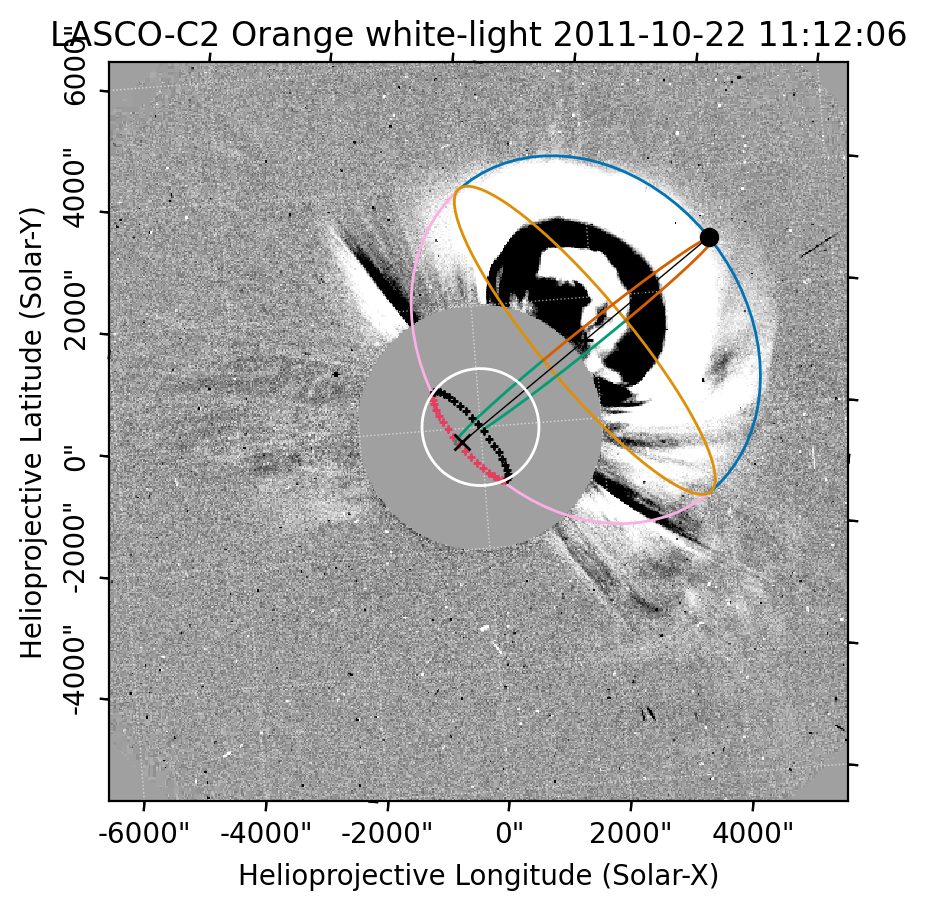
\includegraphics[width=\textwidth]{chapter2/figs/Fig_s1.png}
	\end{subfigure}
	\hfill
	\begin{subfigure}[b]{0.3\textwidth}
		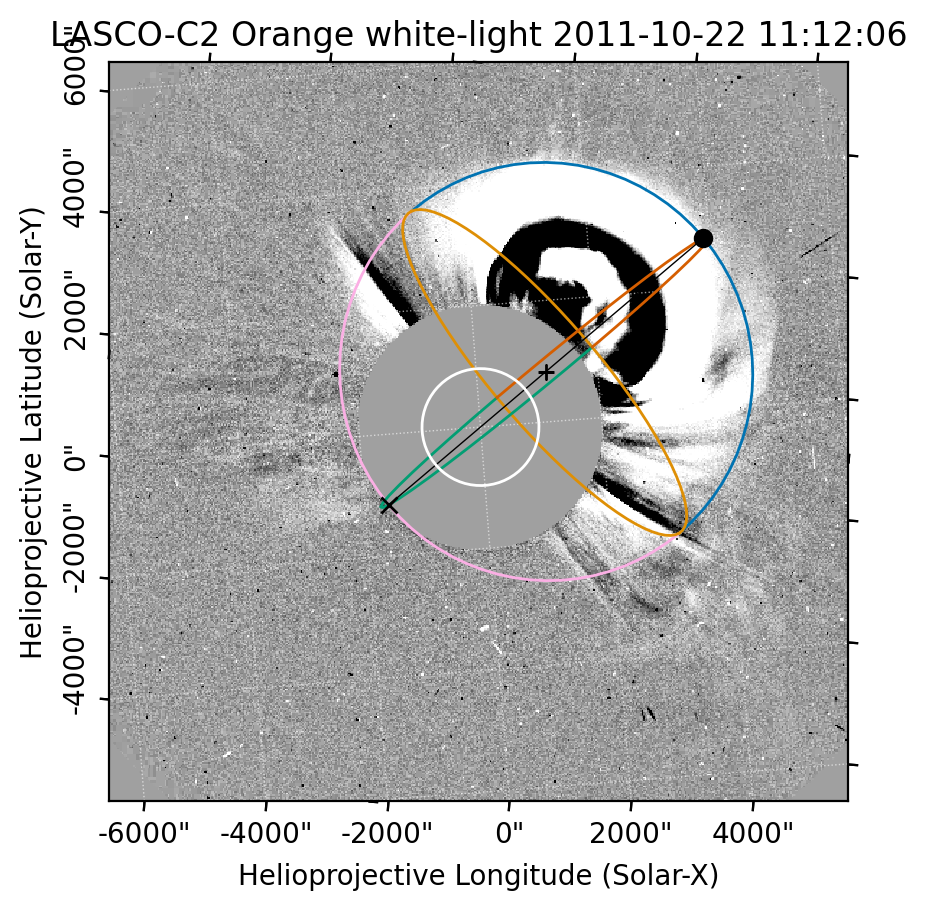
\includegraphics[width=\textwidth]{chapter2/figs/Fig_e1.png}
	\end{subfigure}
	\hfill
	\begin{subfigure}[b]{0.3\textwidth}
		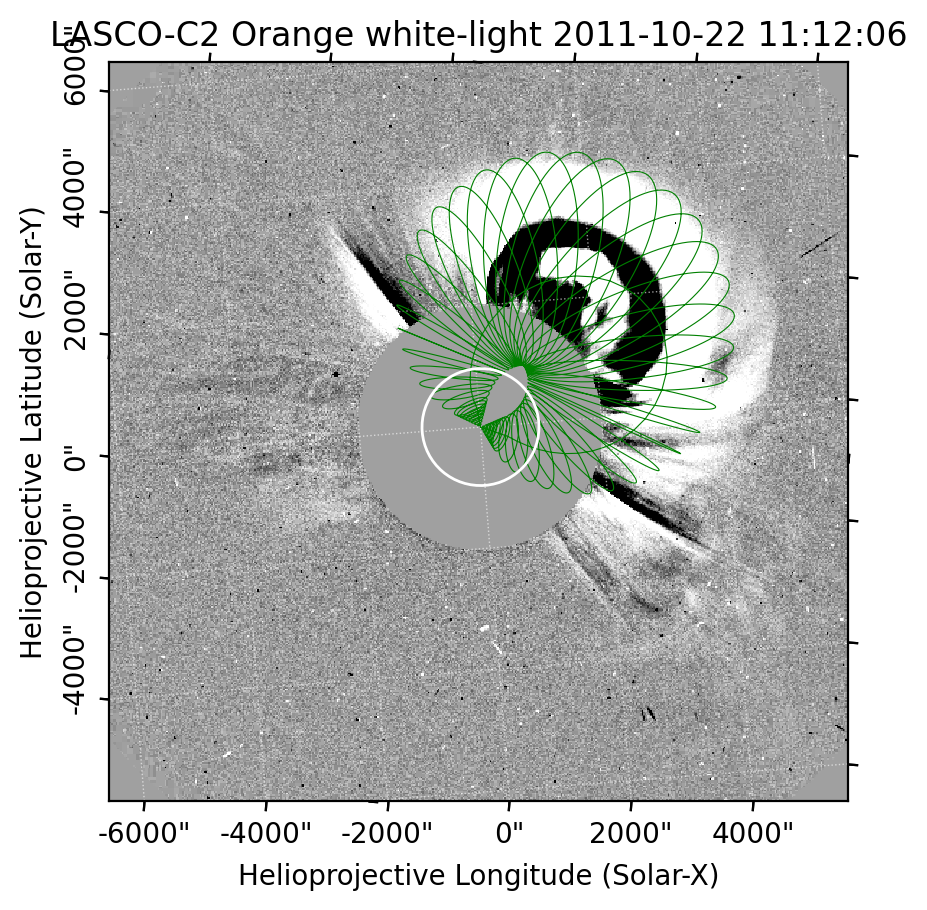
\includegraphics[width=\textwidth]{chapter2/figs/Fig_g1.png}
	\end{subfigure}
	\medskip % Add some vertical space between rows
	\begin{subfigure}[b]{0.3\textwidth}
		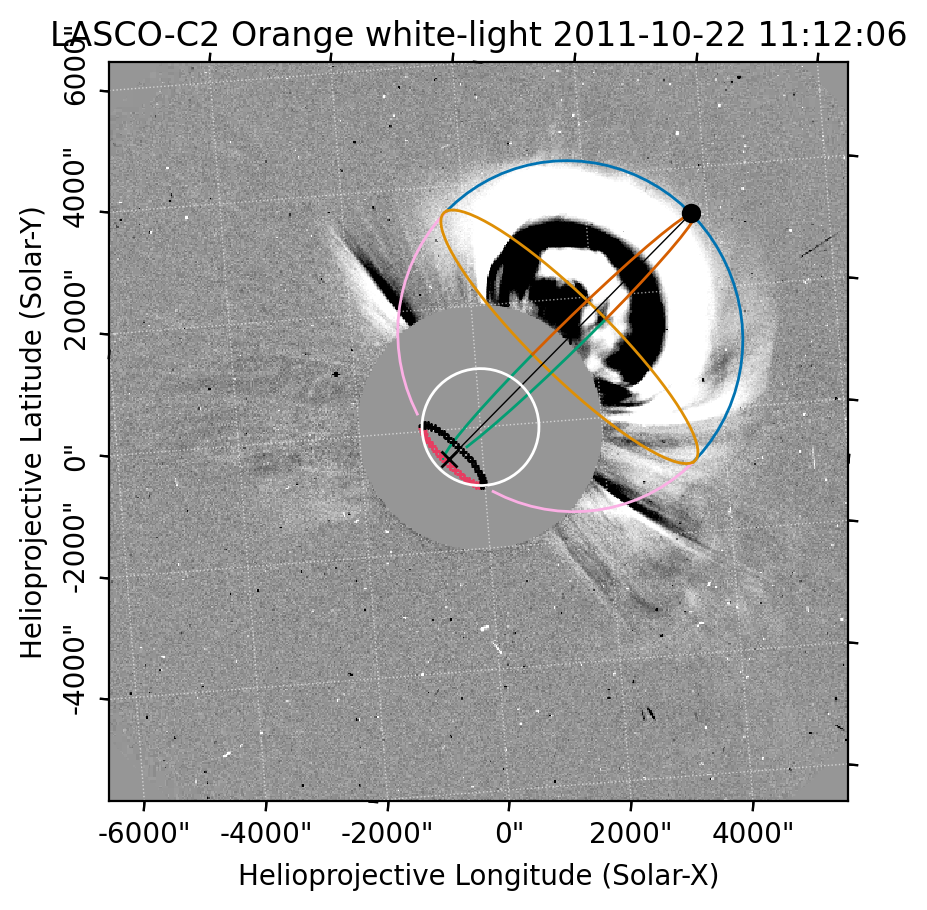
\includegraphics[width=\textwidth]{chapter2/figs/Fig_s2.png}
	\end{subfigure}
	\hfill
	\begin{subfigure}[b]{0.3\textwidth}
		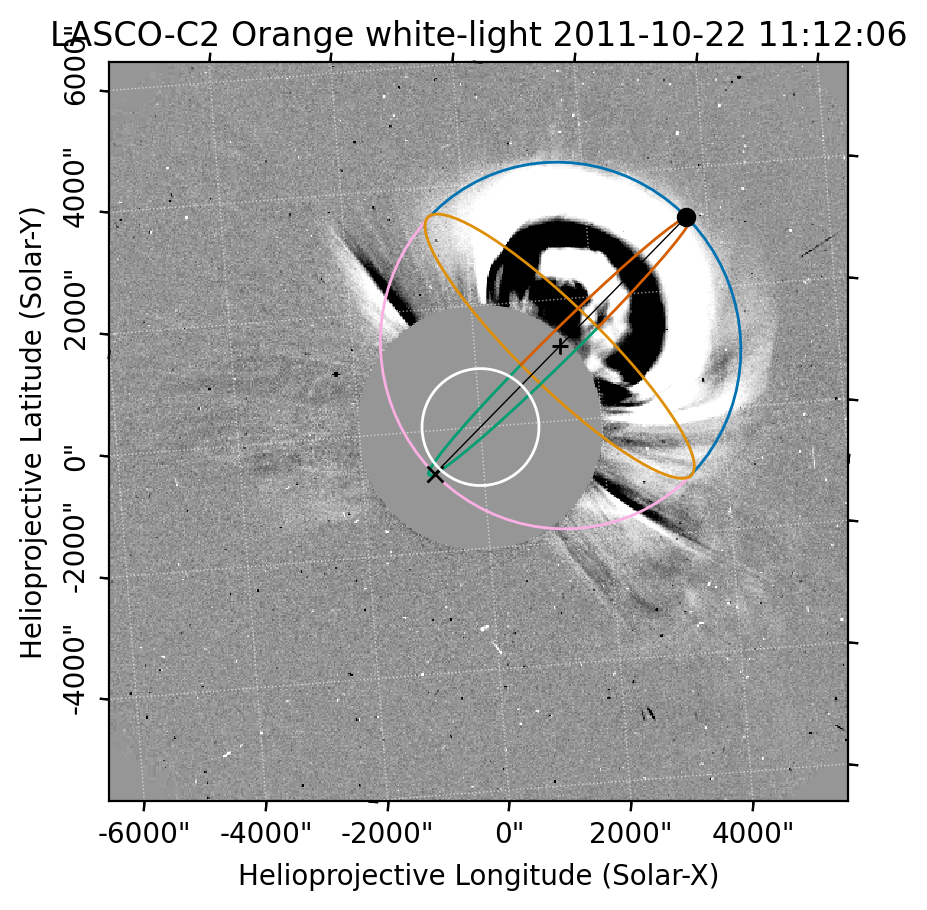
\includegraphics[width=\textwidth]{chapter2/figs/Fig_e2.png}
	\end{subfigure}
	\hfill
	\begin{subfigure}[b]{0.3\textwidth}
		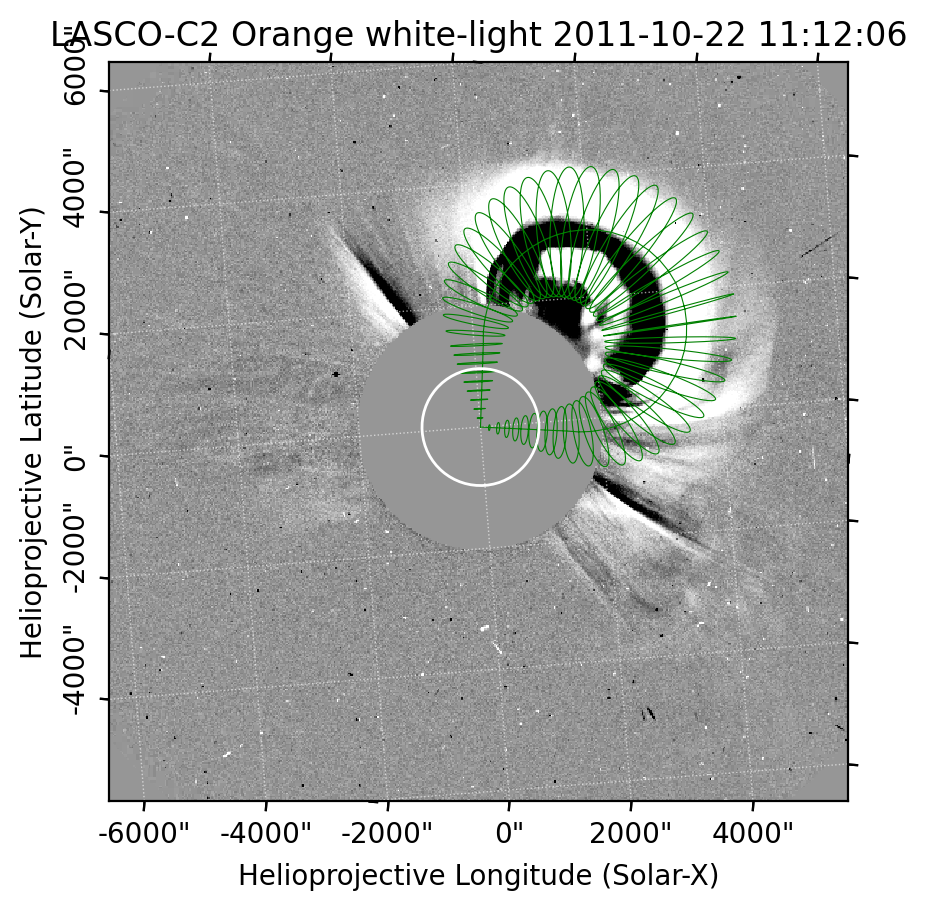
\includegraphics[width=\textwidth]{chapter2/figs/Fig_g2.png}
	\end{subfigure}
	\caption{3D reconstructions of a CME (E03) using the spheroid, ellipsoid, and GCS model from the PyThea tool performed by observers 1 and 2 (top and bottom row, respectively). Credit goes to \citet{miteva_2023}.}
	\label{fig_3D_fit}
\end{figure}

Upon scrutinizing the fitting outcomes for this particular example, it becomes evident that the reconstructions exhibit a discernible bias. The observer's subjective \textit{choice} of structures to align with the model introduces a level of variability. In the top row of Figure~\ref{fig_3D_fit}, distinct shock-related structures (manifested as the bending of streamers) are observed, upon which the idealized GCS flux rope geometry is fitted. Consequently, there is a likelihood of overestimating the CME width. Despite this bias, it is noteworthy that the overall results, including directivity and speed for event E03, are minimally impacted. However, it is acknowledged that the complexity of structure choices can lead to larger discrepancies among different observers.

This study places emphasis on deriving de-projected CME speeds based on fits conducted at two distinct time steps. For each of the three models, the initial CME longitude and latitude are manually specified, utilizing the provided locations of the CME-accompanied SFs. It is important to note that these values exhibit minimal to no substantial changes post-finalization of the fitting procedure. Consequently, the final CME directivity provided by PyThea is considered to be a relatively crude estimate. The ultimate orientations of the CME in IP space and at Earth are derived solely from qualitative information extracted from animations available at this website\footnote{\helioweatherurl}. This approach ensures a rigorous and consistent basis for evaluating the de-projected CME speeds in our analyses.

\subsection{Results}
\subsubsection{Projection Effects}
In our investigation a fitting analysis of approximately 10 CMEs was undertaken by two designated observers within our research team, I was one of the observers. This analysis involved the utilization of all three models available in the PyThea framework, each selected based on the evaluators' individual considerations.

To elucidate, the fitting process was executed at two distinct time steps to derive a velocity parameter based on the height–time estimation. For each specific event, both observers iteratively conducted the 3D de-projection procedure twice, resulting in averaged values for the CME speeds. These values are meticulously presented in Table~\ref{tab_fits}, rounded to the nearest tenth. The disparity between these two fitting instances is denoted as an error (or uncertainty), spanning from 10 \kms to twice the estimated speed. Additionally, Figure 2 illustrates the correlation between 3D speeds and the corresponding estimated errors for each observer. Notably, considerable variability is observed in both plots, particularly concerning the GCS model; nonetheless, a discernible positive trend emerges between the estimated error magnitude and the CME speed.

The inherent subjectivity and diverse levels of experience among observers play a crucial role in the visual fitting procedure. Noteworthy distinctions in evaluated speeds are evident not only between individual observers using the same model (e.g., spheroid fit for E06) but also between a single observer applying different models (e.g., spheroid and GCS for E13). Furthermore, variations in operating system software further contributed to differences in results. Notably, events E04, E08, and E21 were not completed by both observers due to either PyThea computing resource failures or the substantial uncertainty associated with the visual assessment of CME structures.

Our findings underscore the well-established subjectivity inherent in procedures relying on personal judgment for fit quality, where the alignment of structures with the model is subjective. A more comprehensive explanation of this human-in-the-loop bias is detailed in \citep{verbeke_2022}. The specific values of CME speeds are meticulously outlined in Table~\ref{tab_fits}, while their averaged values, categorized by model, as determined by both observers, are presented in Table~\ref{tab_GS_sol}. These averaged values will serve as the basis for subsequent correlation studies.
	
\begin{table}[htp]
	\tiny
	\caption{Parameters of the solar origin, SFs, and CMEs for GSs from Table 1 in \citet{miteva_2023}. All times are in UT, speeds in \kms, AW and MPA in degrees. Credit goes to \citet{miteva_2023}.}
	\label{tab_GS_sol}
	\begin{adjustbox}{width=\textwidth}
		\begin{tabular}{@{}cccccccccccc@{}}
			\toprule
			\textbf{\#} & \textbf{Event} & \textbf{SF} & \textbf{Onset} & \textbf{Location} & \textbf{Time} & \textbf{Speed} & \textbf{AW} & \textbf{MPA} & \textbf{Spheroid} & \textbf{Elliptical} & \textbf{GCS} \\
			(1) & (2) & (3) & (4) & (5) & (6) & (7) & (8) & (9) & (10) & (11) & (12) \\
			\midrule
			\textbf{2011}\\
			E01 & 08-04 & M9.3 & 03:41 & N19W36 & 04:12 & 1315 & 360 & 298 & 1990 & 1920 & 1780 \\
			E02 & 09-24 & M7.1 & 12:33 & N10S56 & 12:48 & 1915 & 360 & 78 & 1570 & 1590 & 1720 \\
			E03 & 10-22 & M1.3 & 10:00 & N25W77 & 10:24 & 1005 & 360 & 311 & 760 & 690 & 840 \\
			\textbf{2012} \\
			E04 & 03-07 & X5.4 & 00:02 & N17S27 & 00:24 & 2684 & 360 & 57 & 2150 & 2460 & 2530 \\
			E05 & \multicolumn{8}{c}{uncertain origin} & - & - & -\\
			E06 & 07-12 & X1.4 & 15:37 & S15W01 & 16:48 & 885 & 360 & 158 & 1060 & 1780 & 1520 \\
			E07 & 09-28 & C3.7 & 23:36 & N06W34 & 24:12 & 947 & 360 & 251 & \multicolumn{3}{c}{multiple CMEs}\\
			E08 & 10-05 & \multicolumn{3}{c}{uncertain} & 02:48 & 612 & 284 & 202 & 350 & 360 & 350 \\
			E09 & 11-09 & \multicolumn{3}{c}{uncertain} & 15:12 & 559 & 276 & 157 & 660 & 570 & 720 \\
			\textbf{2013}\\
			E10 & 03-15 & X1.1 & 05:46 & N11S11 & 07:12 & 1063 & 360 & 112 & 720 & 1040 & 1110 \\
			E11 & \multicolumn{8}{c}{uncertain origin} & - & - & -\\
			E12 & 06-28 & \multicolumn{3}{c}{uncertain} & 02:00 & 1037 & 360 & 214 & \multicolumn{3}{c}{no SOHO images}\\
			\textbf{2014} \\
			E13 & 02-16 & M1.1 & 09:20 & S11E01 & 10:00 & 634 & 360 & 227 & 340 & 690 & 890 \\
			\textbf{2015}\\
			E14 & 01-03 & C1.2 & 03:06 & S05E21 & 03:12 & 163 & 153 & 144 & \multicolumn{3}{c}{no STEREO images} \\
			E15 & 03-15 & C9.1 & 01:15 & S22W25 & 01:48 & 719 & 360 & 240 & \multicolumn{3}{c}{no STEREO images} \\
			E16 & 06-21 & M2.6 & 02:06 & N12E13 & 02:36 & 1366 & 360 & 72 & \multicolumn{3}{c}{no STEREO images} \\
			E17 & \multicolumn{8}{c}{uncertain origin} & - & - & - \\
			E18 & \multicolumn{8}{c}{uncertain origin} & - & - & - \\
			E19 & 12-16 & C6.6 & 08:34 & S13W04 & 09:36 & 579 & 360 & 334 & \multicolumn{3}{c}{no STEREO images} \\
			\textbf{2016} \\
			E20 & 12-28 & M1.8 & 11:20 & S23W11 & 12:12 & 1212 & 360 & 163 & 820 & 680 & 1080 \\
			E21 & 01-14 & \multicolumn{3}{c}{uncertain} & 23:24 & 191 & 360 & 234 & 620 & 440 & 280 \\
			E22 & \multicolumn{8}{c}{uncertain origin} & - & - & - \\
			\textbf{2017}\\
			E23 & 05-23 & \multicolumn{3}{c}{uncertain} & 05:00 & 259 & 243 & 281 & \multicolumn{3}{c}{no SOHO images}\\
			E24 & 09-04 & M5.5 & 20:28 & S11W16 & 20:36 & 1418 & 360 & 184 & 1020 & 1290 & 990 \\
			\textbf{2018}\\
			E25 & 08-20 & \multicolumn{3}{c}{uncertain} & 21:24 & 126 & 120 & 266 & \multicolumn{3}{c}{no STEREO images} \\
			\bottomrule
			\end{tabular}
		\end{adjustbox}
	\end{table}

\begin{table}[htp]
	\caption{CME Speeds (\kms) for Observers 1 and 2. Credit goes to \citet{miteva_2023}.}
	\label{tab_fits}
	\centering
	\begin{tabular}{ccccccc}
		\toprule
		\textbf{\#} & \multicolumn{2}{c}{\textbf{Spheroid}} & \multicolumn{2}{c}{\textbf{Ellipsoid}} & \multicolumn{2}{c}{\textbf{GCS}} \\
		& \textbf{obs1} & \textbf{obs2} & \textbf{obs1} & \textbf{obs2} & \textbf{obs1} & \textbf{obs2} \\
		\midrule
		E01 & $2170\pm870$ & $1800\pm270$ & $2130\pm200$ & $1710\pm450$ & $1590\pm100$ & $1760\pm10$ \\
		E02 & $1780\pm140$ & $1350\pm50$  & $1880\pm580$ & $1310\pm90$ & $1780\pm260$ & $1630\pm130$ \\
		E03 & $770\pm40$ & $740\pm10$ & $640\pm180$ & $740\pm180$ & $1020\pm170$ & $700\pm270$ \\
		E04 & - & $2150\pm140$ & - & $2460\pm70$ & - & $2530\pm630$ \\
		E06 & $1410\pm420$ & $710\pm70$ & $1870\pm50$ & $1700\pm300$ & $1680\pm870$ & $1560\pm470$ \\
		E08 & $350\pm90$ & - & $360\pm150$  & - & $350\pm70$ & - \\
		E09 & $690\pm280$ & $630\pm150$ & $550\pm170$  & $590\pm60$ & $670\pm610$ & $710\pm220$ \\
		E10 & $840\pm380$ & $610\pm1040$ & $1120\pm360$ & $960\pm90$ & $1160\pm650$ & $1310\pm80$ \\
		E13 & $320\pm90$ & $350\pm50$ & $620\pm140$ & $750\pm160$ & $780\pm80$ & $1310\pm700$ \\
		E20 & $830\pm190$ & $800\pm600$ & $790\pm90$ & $570\pm20$ & $1240\pm280$ & $1130\pm230$ \\
		E21 & $620\pm230$ & - & $440\pm40$ & - & $280\pm180$ & - \\
		E24 & $750\pm270$ & $1310\pm220$ & $880\pm350$ & $2020\pm960$ & $950\pm120$ & $1560\pm540$ \\
		\bottomrule
	\end{tabular}
\end{table}

\subsubsection{Correlation between GSs, Coronal and Near-Sun Parameters}
In Figure 3, we present a scatter plot depicting the relationship between the modulus of the GS Dst index and the CME speed, as derived from the data in Table~\ref{tab_GS_sol}. To enhance clarity, the averaged results of the three model fits are collectively illustrated and labeled as '3D-mean' in Table 4. These values are juxtaposed with the 2D SOHO-LASCO CME speed. Horizontal lines, representing the error estimates from the 3D de-projections, are also included for completeness, despite the substantial overlap. For demonstrative purposes, we highlight the largest error value among the two observers, as outlined in Table 3.

The analysis conducted reveals no discernible trend between the Dst index and the CME speed, irrespective of whether the 3D de-projection or the 2D CME speeds are considered. It is important to note that, due to data constraints, 3D speed de-projections were not feasible for the most robust GSs. This limitation results in a skewed distribution of the 3D speeds, impacting the overall findings. Despite the modest sample size (comprising between 10 and 20 event pairs), the quality of the fit is assessed through Pearson correlations. The correlation coefficients, reflecting the relationship between all CME speed estimations and the GS Dst index, are systematically documented in Table 4. These coefficients range from negligible (e.g., 0.04 for the 2D LASCO speeds) to moderate (with the highest value reaching 0.55, observed with the GCS model). Importantly, no significant correlations are identified between the Dst index and other coronal parameters, such as SF class, location, and CME AW, as inclusively presented in the same table for comprehensive evaluation.

\subsubsection{Correlation between GSs and IP Parameters}
Here, we explore the correlations between Geospace Storms (GSs) and various parameters associated with pre-selected Interplanetary (IP) phenomena. To visually represent these relationships, scatter plots are employed for specific parameter pairs, as follows: the Dst index versus Interplanetary Coronal Mass Ejection (ICME) speed and IP shock speed in Figure 4; Dst versus Mach number and sheath duration in Figure 5; Dst versus jBzj and Bd/Bu in Figure 6; and Dst versus Td/Tu and Nd/Nu in Figure 7. The corresponding Pearson correlation values elucidating these trends are documented in Table 5.

For the limited sample of GS storms utilized in our analyses, we observe a moderately positive trend between the Dst index and the plasma compression parameters at the shock interface (downstream to upstream ratio). Interestingly, these correlations are comparable to, or slightly larger than, those obtained when considering ICME speeds from the Wind and ACE spacecraft. Notably, the trend with jBzj is weaker (0.37 for our dataset), in contrast to the robust trend reported in previous studies. Furthermore, the correlations involving Dst and IP shock speed, Mach number, or sheath duration are relatively smaller.

Recent reports have highlighted strong correlations with different components of the electric and magnetic fields [12], although this aspect exceeds the scope of our current analyses. It is essential to exercise caution in interpreting these results, given the absence of uncertainty estimates for the correlation coefficients.

The ICME and IP shock catalogs employed in our study offer additional parameters, including averaged magnetic field B, plasma speed V inside the magnetic structure, and upstream plasma beta bu (not presented in Table 1). However, no robust correlations emerge between these parameters and the Dst index, with all correlation coefficients found being smaller than 0.2.

\subsubsection{On the GS Strength Forecasting Based on Solar and IP Parameters}
We examine the collective impact of magnetic obstacle type and orientation upon Earth arrival (columns 5 and 9 from Table 1), along with the 3D reconstructed Coronal Mass Ejection (CME) speeds (columns 10–12 from Table 2), on the intensity of Geospace Storms (GSs), approximated in this study using the Dst index.

The most potent GSs in our compilation, arranged in descending order based on their Dst values (nT), exhibit distinctive magnetic structure parameters, including complexity, orientation of arrival, and speed at Earth (refer to Tables 1 and 2):

- E15 (-234): Magnetic obstacle type undefined, fast speed (f), no 3D speed estimation
- E16 (-198): Complex (Cx) structure, nose-like (n) orientation, no 3D speed estimation
- E25 (-175): Flux-rope (Fr) structure, nose-like (n) orientation, no 3D speed estimation
- E19 (-166): Flux-rope (Fr) structure, nose-like (n) orientation, no 3D speed estimation
- E03 (-147): Complex (Cx) structure, fast speed (f), reduced 3D speed compared to 2D
- E04 (-145): Complex (Cx) structure, nose-like (n) orientation, similar 3D speed compared to 2D
- E06 (-139): Flux-rope (Fr) structure, nose-like (n) orientation, larger 3D speed compared to 2D
- E10 (-132): Flux-rope (Fr) structure, nose-like (n) orientation, similar 3D speed compared to 2D

Upon scrutiny of these cases, it becomes apparent that the most intense GSs are linked to magnetic obstacles characterized by a nose-like (n) orientation upon arrival, coupled with either a complex (Cx) or flux-rope (Fr) structure. Exceptions include instances of fast speed flank hits or flank hits in combination with a complex (Cx) structure. It has been established that sheath duration does not serve as a decisive ordering parameter. Other GSs of lesser intensity (refer to Table 1) predominantly result from flank hits or exhibit uncertain configurations, possibly influenced by fast solar wind streams or Corotating Interaction Regions (CIRs). Notably, E20 is an exception, resulting from a nose hit; however, the Interplanetary (IP) structure associated with it has a notably low speed, as observed in the examined animations.

It is crucial to acknowledge that the IP shock speed provided by the Wind and ACE satellites represents a single point sample within the entire structure. In contrast, animations offer a global speed distribution. Therefore, our interpretation considers information from both sources — speed reconstructions and in situ measurements — to enhance the robustness of our analysis.

\subsection{Discussion}
In this study, we conduct post-event analyses of all geo-effective storms observed during solar cycle 24 with the aim of identifying distinct and reliable predictors for GS intensity. The overarching objective is to derive dependable solar or near-Sun parameters from remote sensing image data that can be effectively utilized for early warnings regarding potential GS onsets and their strength. Our approach involves the integration of solar, near-Sun, and interplanetary parameters, primarily sourced from catalogs but also subject to our analysis using space-related databases. Notably, we incorporate the results obtained from a novel tool for CME speed de-projection, termed PyThea, which is employed for the first time alongside well-established parameters in space weather and geophysics research.

Among the solar and near-Sun phenomena considered, certain selected parameters exhibit a positive correlation with the Dst index. Notably, the correlation coefficient, when comparing the observed projected CME speed, experiences an improvement from 0.04 (as obtained from LASCO) to a range of 0.34–0.55, achieved through various geometrical models provided by the PyThea software package, combining LASCO and STEREO data. However, our exploration of different CME geometry reconstruction techniques reveals a susceptibility to large speed errors, particularly in the case of fast CMEs. This aligns with findings from prior studies focusing on CME arrival time and speed forecasts for Earth, suggesting a potential overestimation of CME launch speed for fast events, likely attributable to the increased complexity in discerning coronal structures due to the rapid expansion of the magnetic structure associated with the CME.

Moreover, our examination indicates that fast halo CMEs may exhibit significant deviations, stemming from the overlap in shock and magnetic structure components, thereby strongly impacting the reconstruction quality. Consequently, we assert that the derived near-Sun 3D parameters continue to possess limited forecasting potential for predicting GS strength. In contrast, most selected IP parameters derived from in situ measurements display moderate positive correlations with GS strength, in line with expectations. However, the Bz parameter (southward component of the magnetic field) shows a relatively low correlation coefficient of 0.37, possibly influenced by the limited event sample used in our study.

Other IP parameters, such as ICME and IP shock speeds, along with their derivative parameters (e.g., Mach number), exhibit a positive trend with the Dst index, featuring correlation coefficients of 0.35–0.45. Nevertheless, none of these parameters emerge as predominant, and their reliance on single-point in situ observation raises considerations about their comprehensive predictive capability. Discrepancies in ICME speed values between ACE and Wind measurements prompt further investigation, with slightly stronger correlation coefficients (0.4–0.5) observed when utilizing different shock parameters. However, averaged values of magnetic field and speed within the magnetic structure, plasma beta in the upstream region, or duration of the sheath region show no correlation with GS strength.

Among the multitude of considered solar, near-Sun, and IP parameters, only the combination of speed and orientation (nose-like) of the magnetic obstacle appears to exert a positive influence on GS strength, as indicated by qualitative results obtained from animations accessible at \textit{helioweather}. Consistent with earlier studies, de-projected CME speeds emerge as imperative for enhancing modeling accuracy when predicting CME propagation through the IP space. However, a notable observation is the apparent lack of direct impact of 3D de-projected CME speed on GS intensity. Consequently, an accurate estimation of the ICME speed distribution over the entire ICME structure upon arrival at Earth assumes significant importance. We emphasize the imperative need for permanent stereoscopic observations, exemplified by the upcoming ESA Vigil mission situated at Lagrange point L5. Future research endeavors should aim for a more comprehensive disentanglement of distinct CME structures, thereby enabling more reliable 3D reconstructions of CME geometries for a nuanced estimation of 3D speed and directivity.































































